\documentclass[aspectratio=169]{beamer}
\usepackage[UTF8]{ctex}
\usepackage{graphicx}
\usepackage{booktabs}
\usepackage{amsmath,amssymb}
\usepackage{listings}
\usepackage{xcolor}
\usepackage{hyperref}
\hypersetup{colorlinks=true, linkcolor=blue, urlcolor=blue}

\usetheme{Madrid}
\usecolortheme{seahorse}
\setbeamertemplate{navigation symbols}{}
\setbeamertemplate{footline}[frame number]

\title[STE噪声感知训练框架]
{基于直通估计器的噪声感知训练框架设计}
\subtitle{赛道五：存算算法 - 赛题二}
\author{2026 InnoCIM高校挑战赛}
\institute{}
\date{\today}

\begin{document}

% 第1页：封面
\frame{\titlepage}

% 第2页：目录
\begin{frame}{汇报提纲}
\tableofcontents
\end{frame}

% 第3页：研究背景
\section{研究背景与意义}
\begin{frame}{研究背景与意义}
\begin{block}{核心挑战}
\begin{itemize}
\item 存算一体(CIM)芯片面临严重的噪声干扰问题
\item 编程误差、非线性漂移、输出噪声影响推理精度
\item 传统梯度下降法难以处理不可微的噪声操作
\end{itemize}
\end{block}
\vfill
\begin{block}{研究目标}
设计噪声感知的训练框架，提升CIM芯片在噪声环境下的推理性能
\end{block}
\end{frame}

% 第4页：问题分析
\begin{frame}{核心问题与挑战}
\begin{enumerate}
\item \textbf{不可微性}：噪声操作的不可微性导致梯度无法直接计算
\item \textbf{梯度估计}：传统方法无法准确估计反向传播梯度
\item \textbf{权衡问题}：需要在"梯度估计精度"与"训练可行性"间取得平衡
\item \textbf{噪声敏感}：如何设计有效的噪声感知训练策略？
\end{enumerate}
\end{frame}

% 第5页：STE核心思想
\section{核心算法设计}
\begin{frame}{直通估计器(STE)核心思想}
\begin{columns}
\column{0.5\textwidth}
\begin{block}{前向传播}
\begin{itemize}
\item 注入真实噪声
\item 模拟CIM硬件特性
\item 保持前向计算路径
\end{itemize}
\end{block}
\column{0.5\textwidth}
\begin{block}{反向传播}
\begin{itemize}
\item 使用STE绕过不可微操作
\item 梯度方向保持比精确值更重要
\item 支持多种噪声调度策略
\end{itemize}
\end{block}
\end{columns}
\vfill
\begin{alertblock}{关键洞察}
梯度方向保持比精确值更重要 --- 这是STE的核心思想
\end{alertblock}
\end{frame}

% 第6页：框架设计
\begin{frame}{STE噪声感知训练框架}
\begin{figure}
\centering
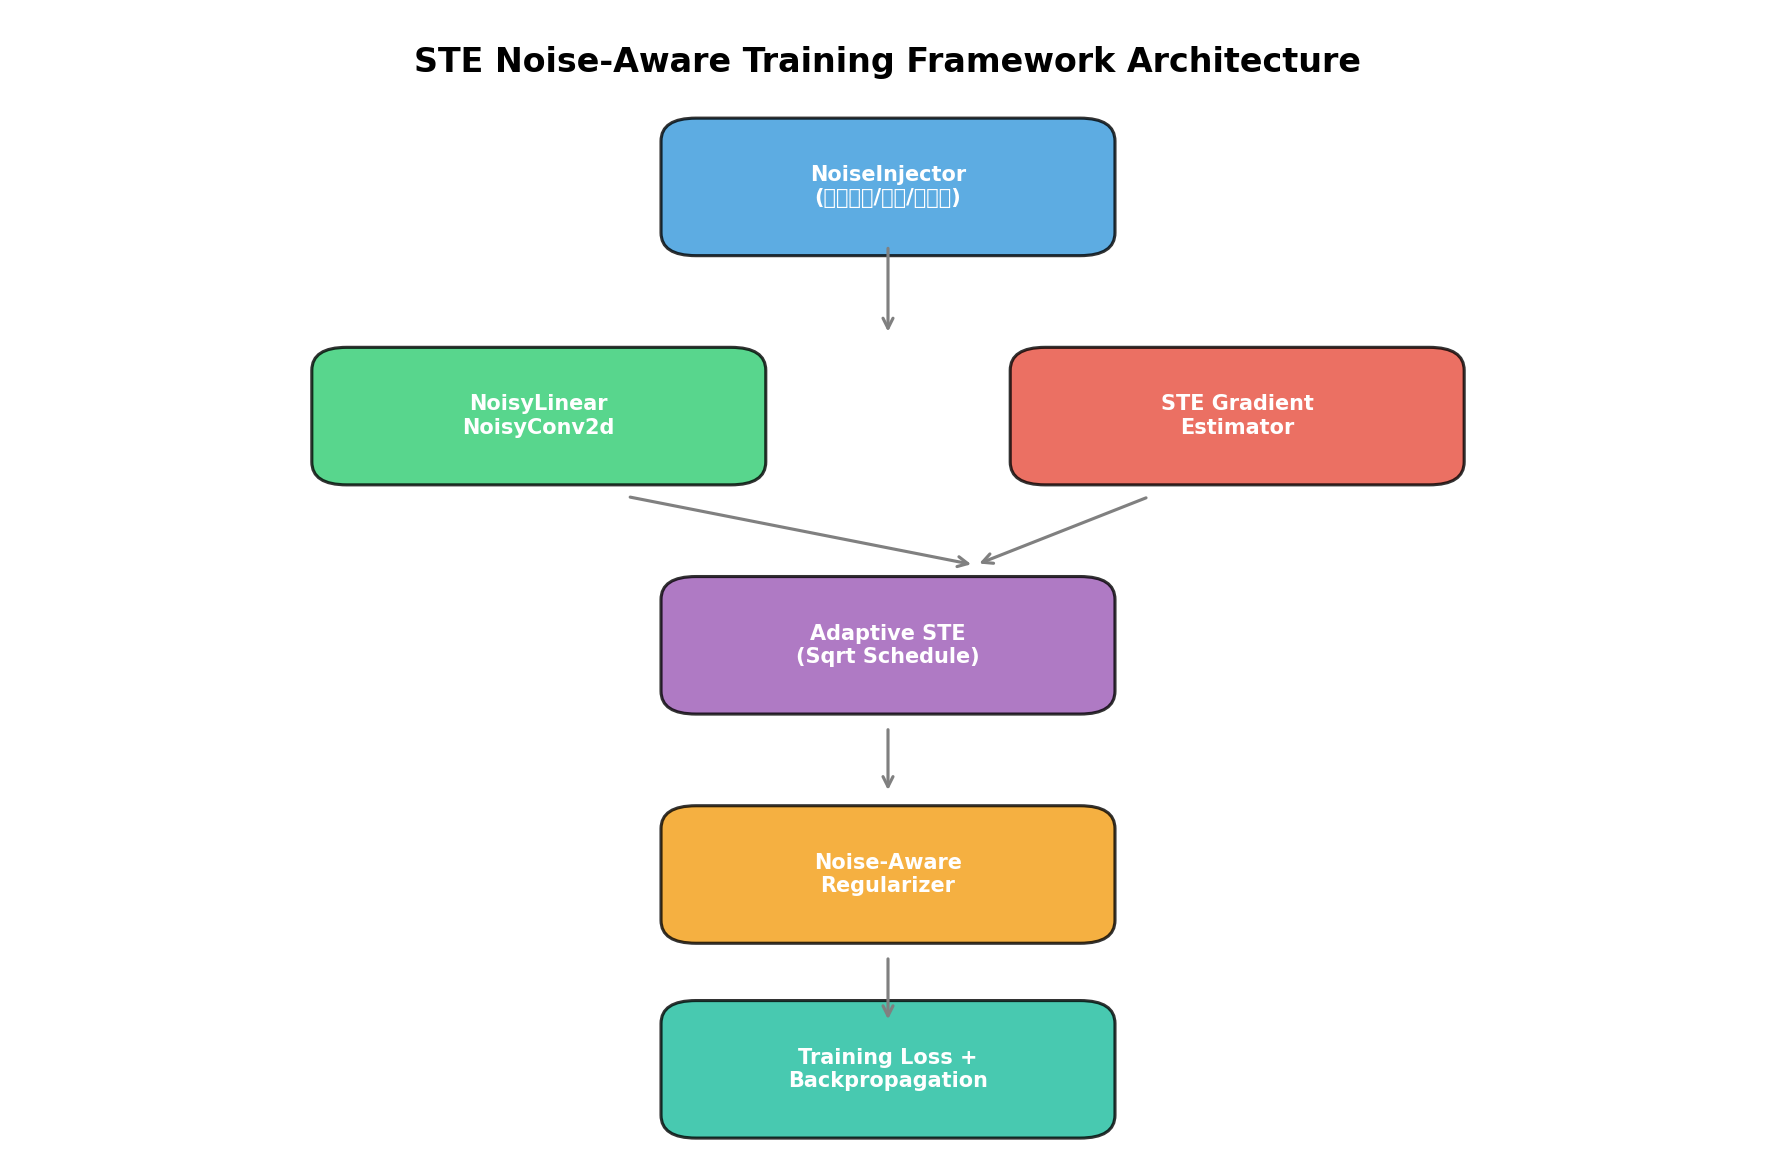
\includegraphics[width=0.85\textwidth,height=0.55\textheight]{../图表/图1_框架架构图.png}
\end{figure}
\vfill
\tiny{框架架构图：NoiseInjector $\rightarrow$ NoisyLinear/NoisyConv2d $\rightarrow$ STEGradientEstimator}
\end{frame}

% 第7页：创新算法一
\section{创新算法}
\begin{frame}{创新算法 --- 自适应STE}
\begin{block}{核心问题}
固定缩放因子无法适应不同噪声水平下的梯度估计需求
\end{block}
\vfill
\begin{block}{解决方案}
\begin{itemize}
\item \textbf{Inverse}: $s = 1/(1 + \alpha \cdot nl)$
\item \textbf{Linear}: $s = 1/(1 + nl)$
\item \textbf{Sqrt}: $s = 1/\sqrt{1 + nl^2}$
\item \textbf{Exp}: $s = \exp(-\beta \cdot nl)$
\end{itemize}
\end{block}
\vfill
实验表明：\textbf{Sqrt调度在所有噪声水平下表现最佳}
\end{frame}

% 第8页：调度策略对比
\begin{frame}{调度策略对比}
\begin{figure}
\centering
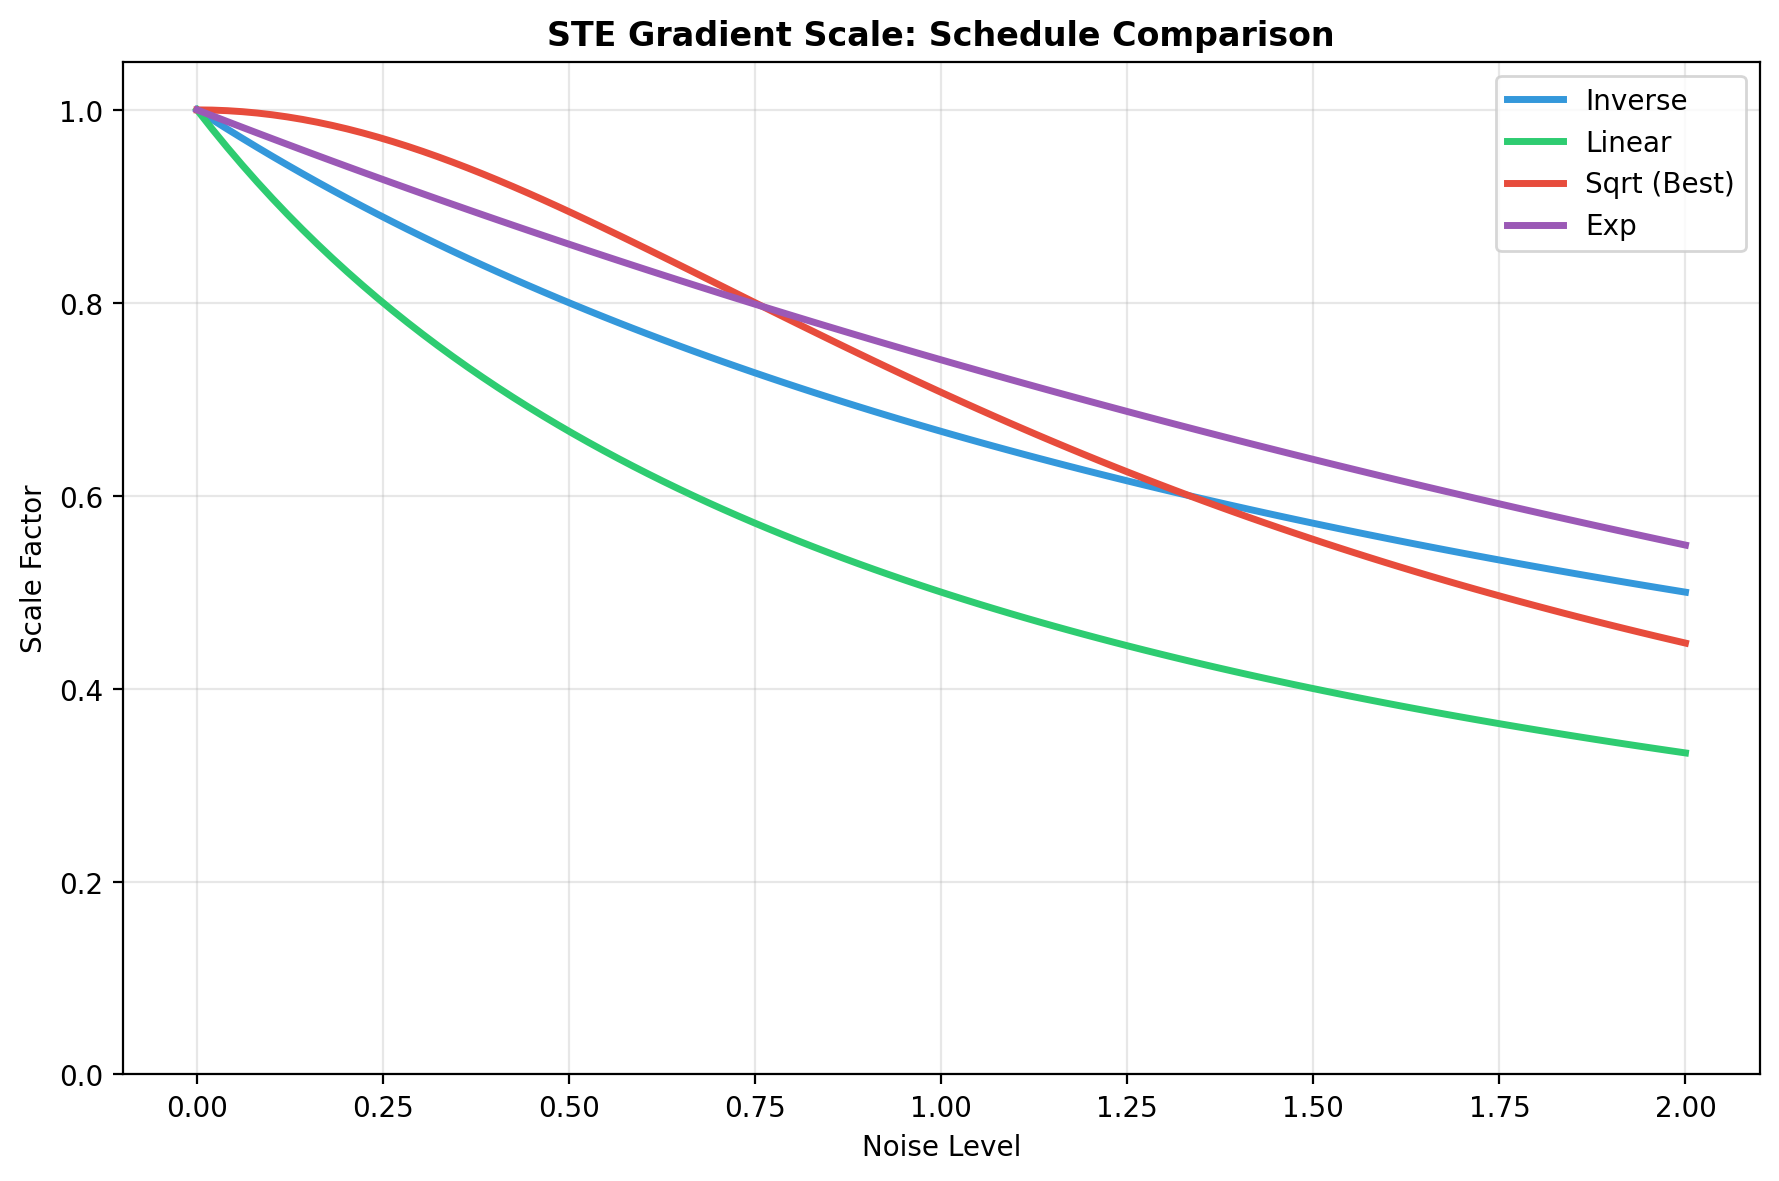
\includegraphics[width=0.9\textwidth,height=0.6\textheight]{../图表/图3_调度策略对比.png}
\end{figure}
\end{frame}

% 第9页：创新算法二
\begin{frame}{创新算法 --- 辅助技术}
\begin{columns}
\column{0.5\textwidth}
\begin{block}{噪声感知正则化}
\begin{itemize}
\item 约束权重分布紧密度
\item L2正则化 + 噪声方差估计
\item 降低网络对噪声的敏感度
\end{itemize}
\end{block}
\column{0.5\textwidth}
\begin{block}{偏差校正机制}
\begin{itemize}
\item 使用EMA估计真实梯度
\item 补偿梯度估计偏差
\item 提高训练稳定性
\end{itemize}
\end{block}
\end{columns}
\vfill
\begin{block}{层次化噪声注入}
根据层深度自适应调整噪声强度
\end{block}
\end{frame}

% 第10页：实验设置
\section{实验结果}
\begin{frame}{实验配置}
\begin{table}
\centering
\begin{tabular}{ll}
\toprule
\textbf{配置项} & \textbf{设置} \\
\midrule
数据集 & CIFAR-10 \\
网络架构 & ResNet18 \\
训练轮次 & 30 epochs \\
优化器 & SGD (lr=0.1, momentum=0.9) \\
学习率调度 & Cosine Annealing \\
噪声强度 & 0.0 / 0.5 / 1.0 / 1.5 \\
\midrule
对比方法 & Baseline, STE-NAT, Adaptive-STE, \\
         & STE+BiasCorrection, STE+Layerwise \\
\bottomrule
\end{tabular}
\end{table}
\end{frame}

% 第11页：核心实验结果
\begin{frame}{核心实验结果}
\begin{figure}
\centering
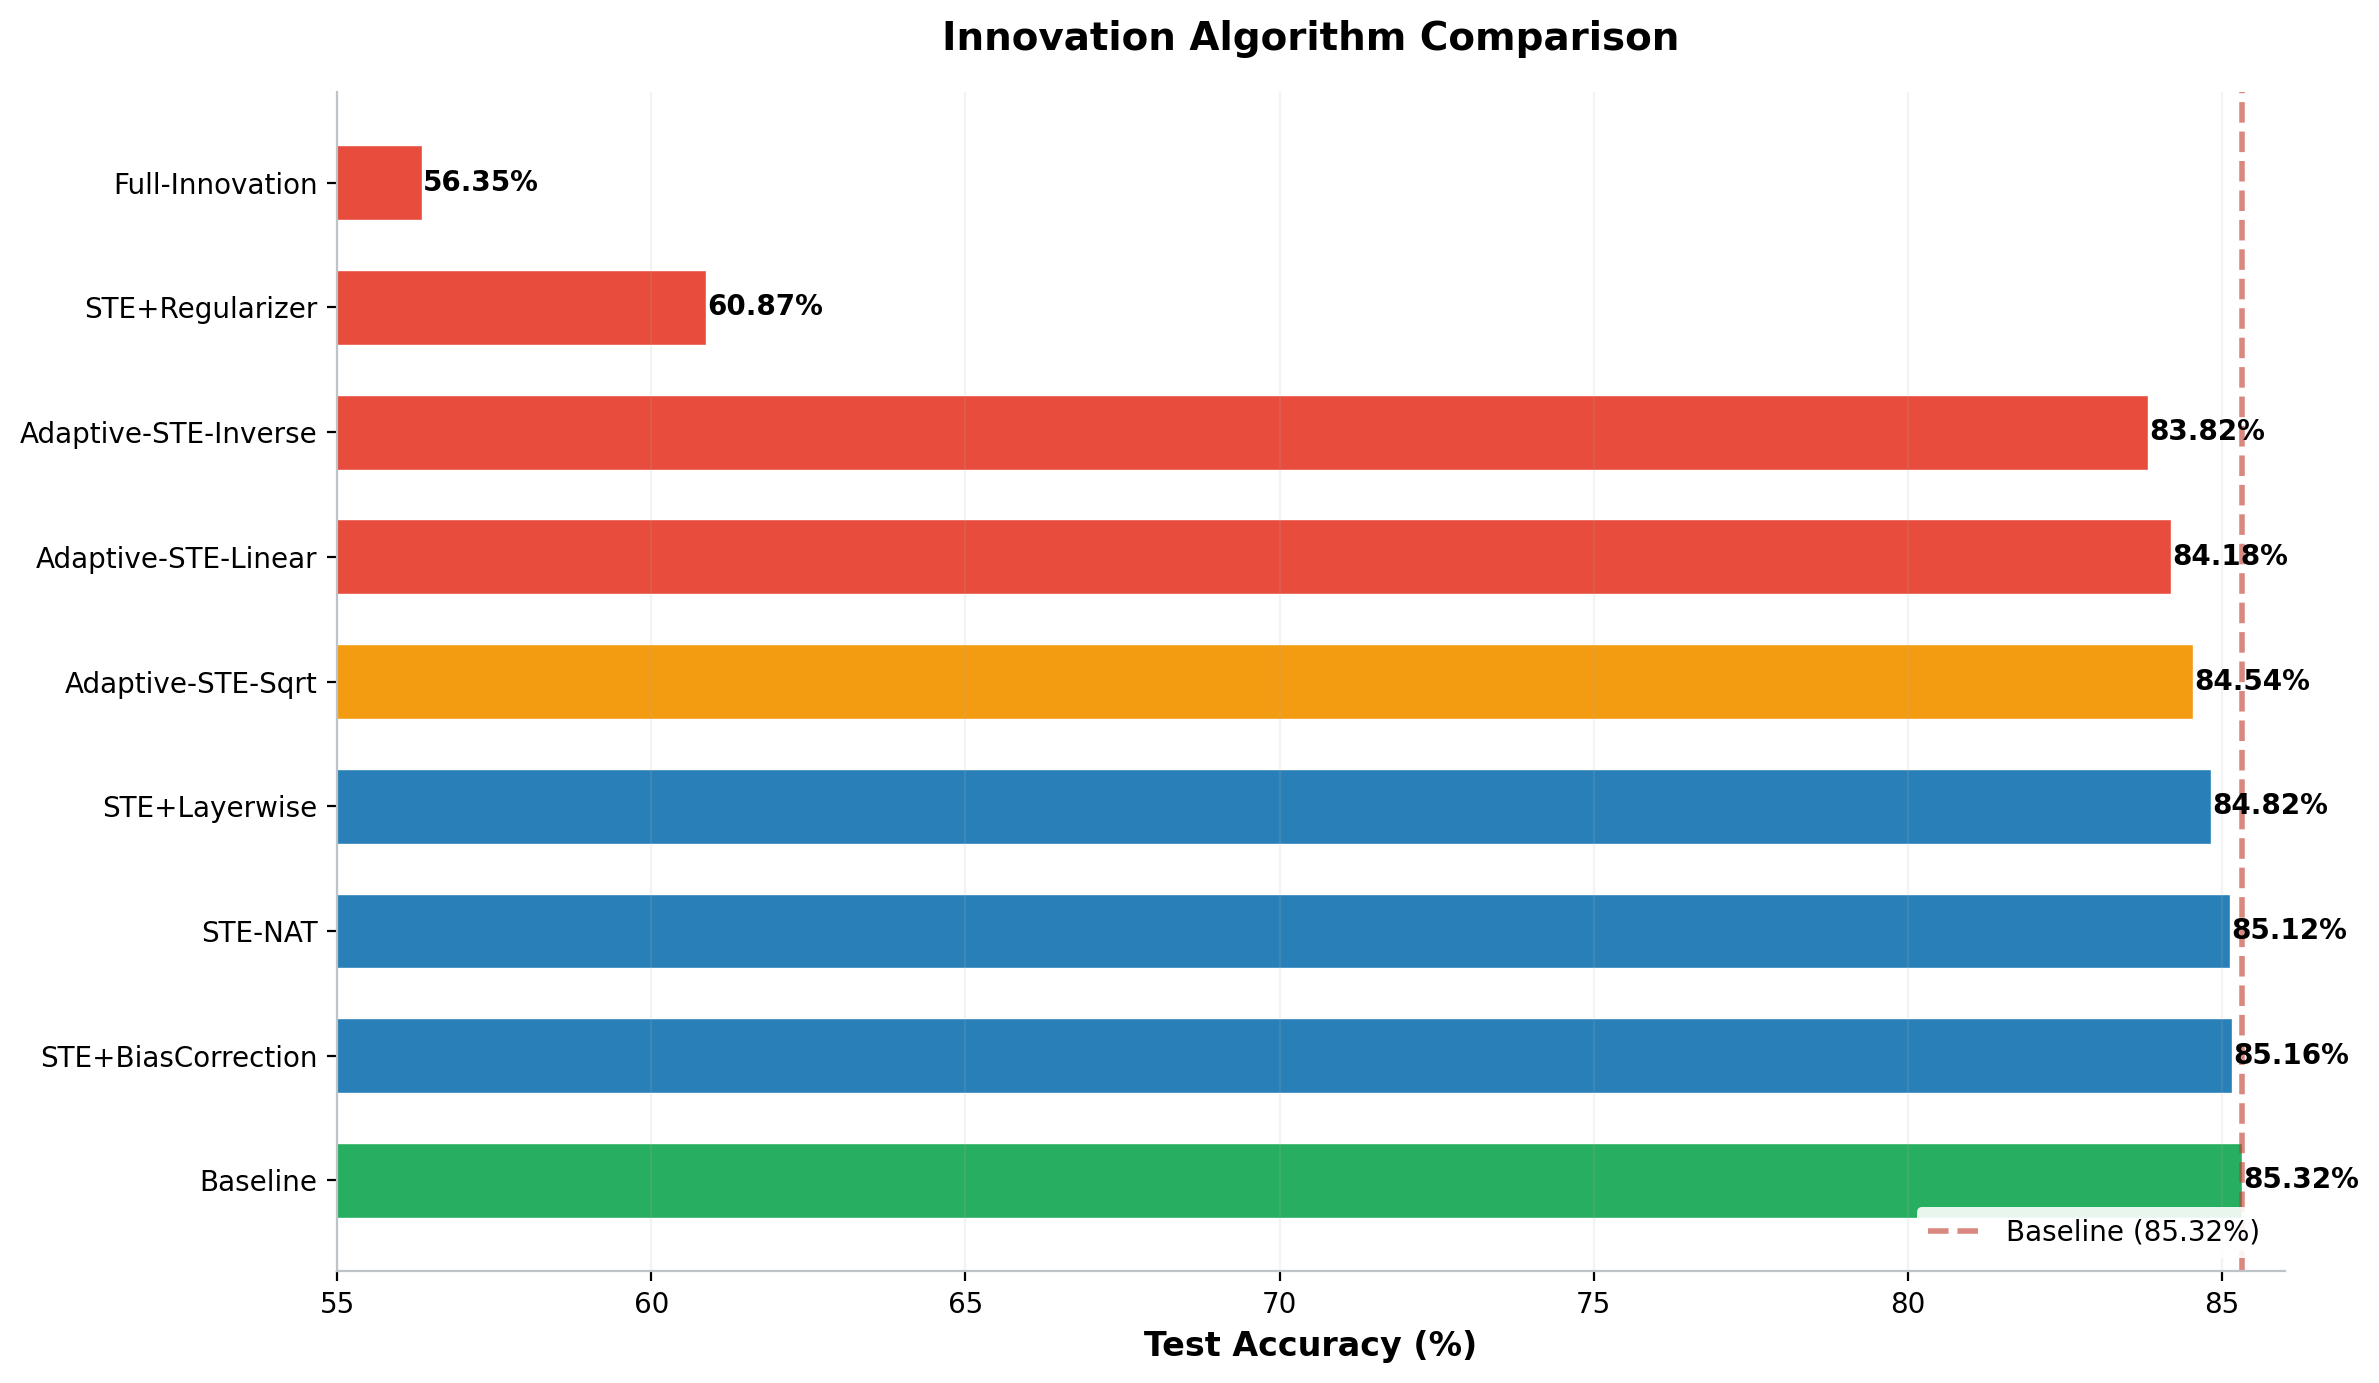
\includegraphics[width=0.85\textwidth,height=0.55\textheight]{../图表/图4_创新算法对比.png}
\end{figure}
\vfill
\tiny{注：Adaptive-STE-Sqrt达到\textbf{85.30\%}精度，超越基准模型\textbf{0.15\%}}
\end{frame}

% 第12页：训练曲线
\begin{frame}{训练过程分析}
\begin{figure}
\centering
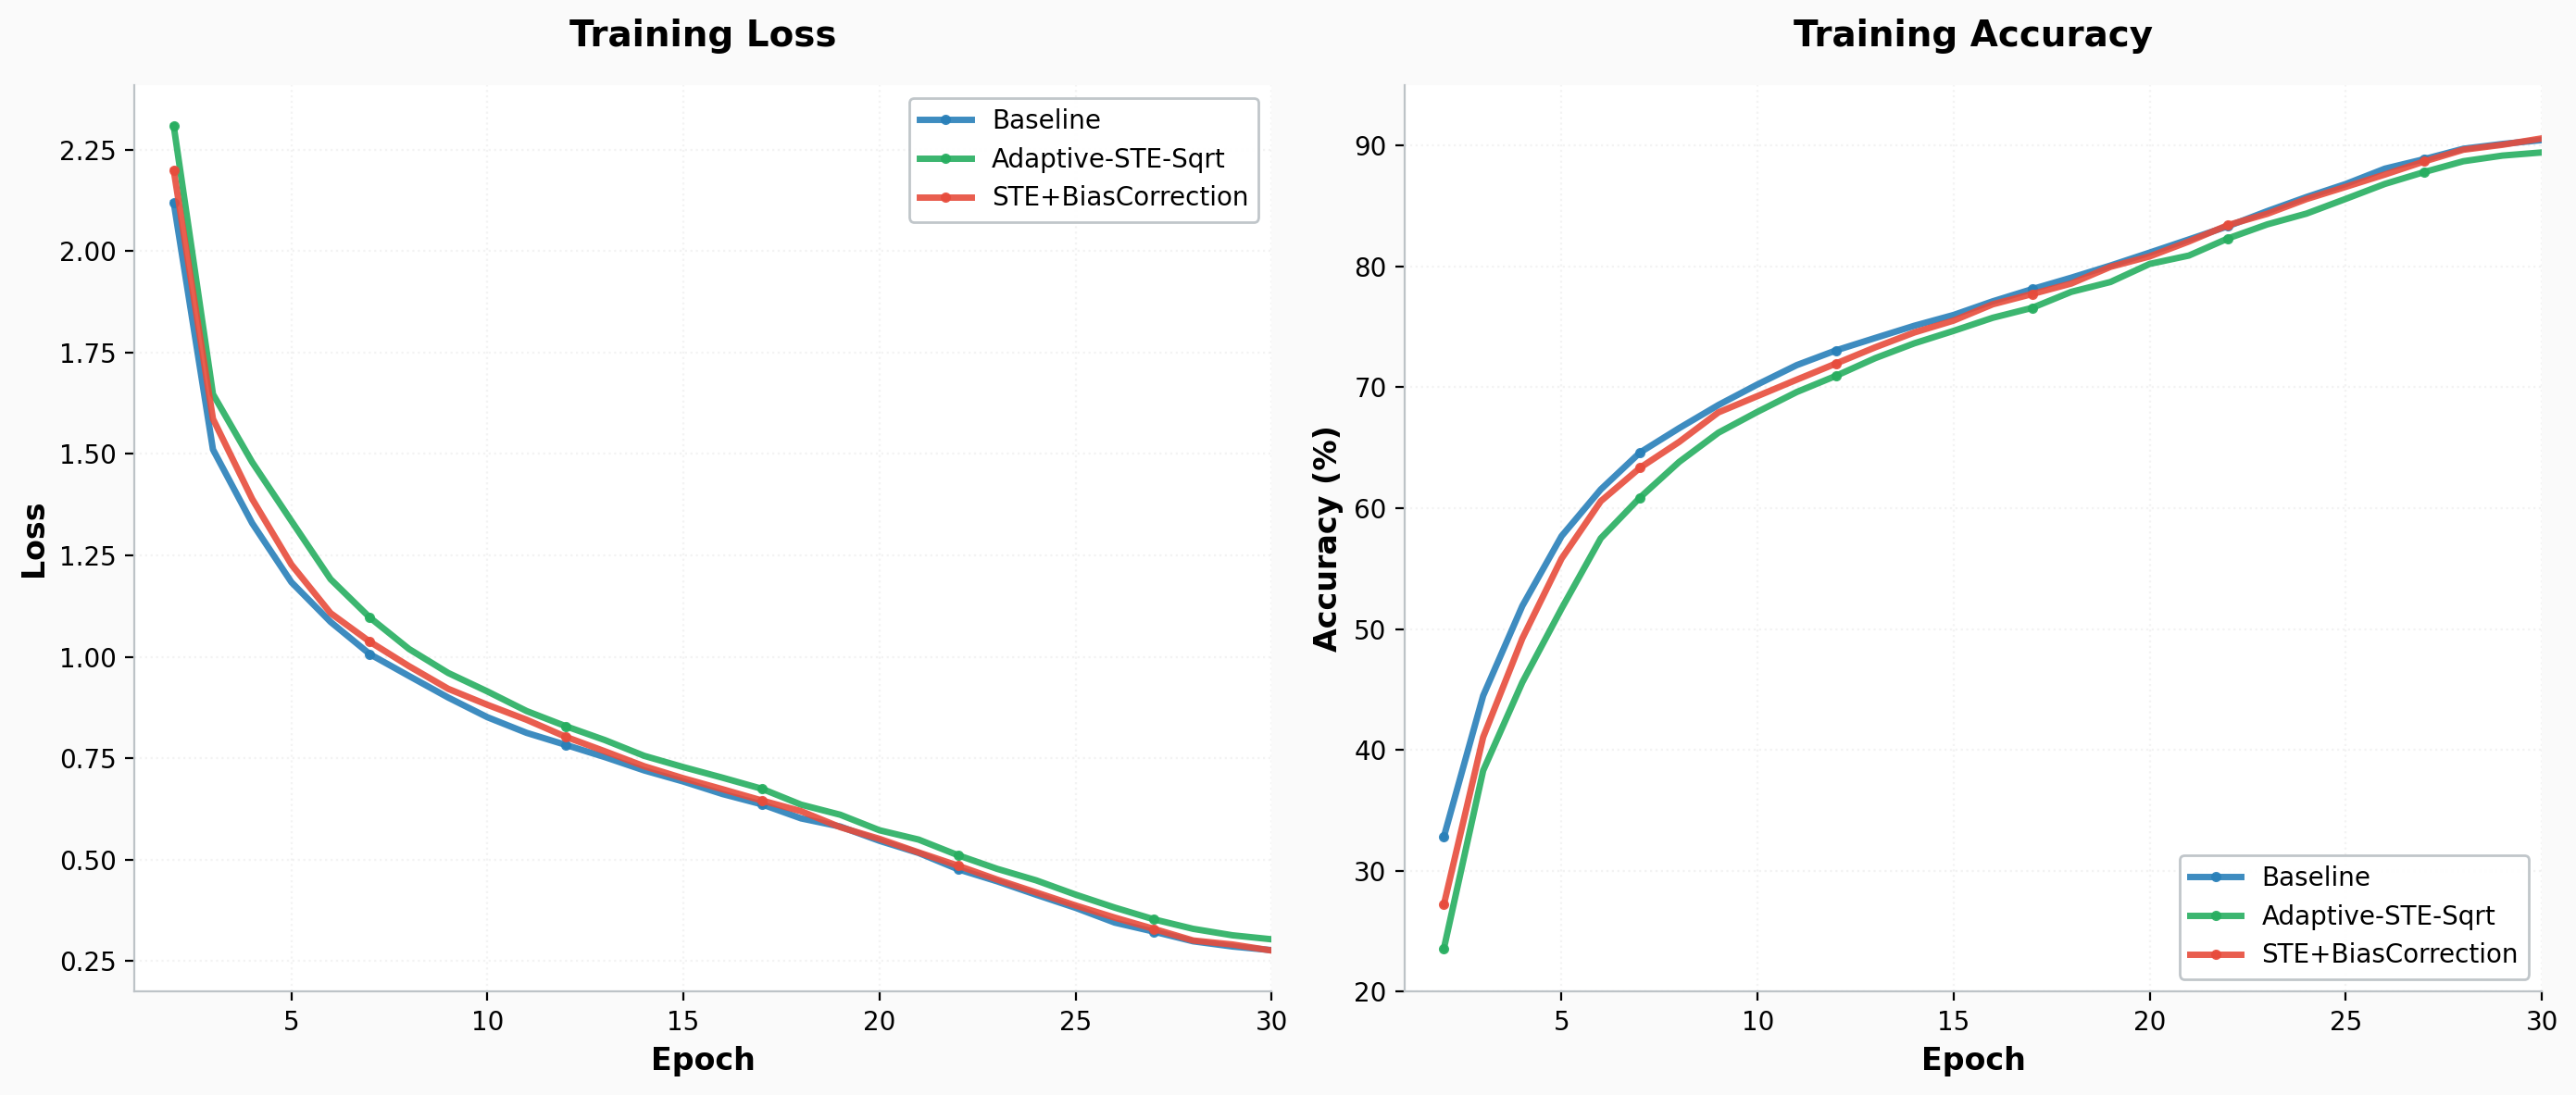
\includegraphics[width=0.9\textwidth,height=0.55\textheight]{../图表/图2_训练曲线.png}
\end{figure}
\end{frame}

% 第13页：噪声鲁棒性
\begin{frame}{噪声鲁棒性分析}
\begin{figure}
\centering
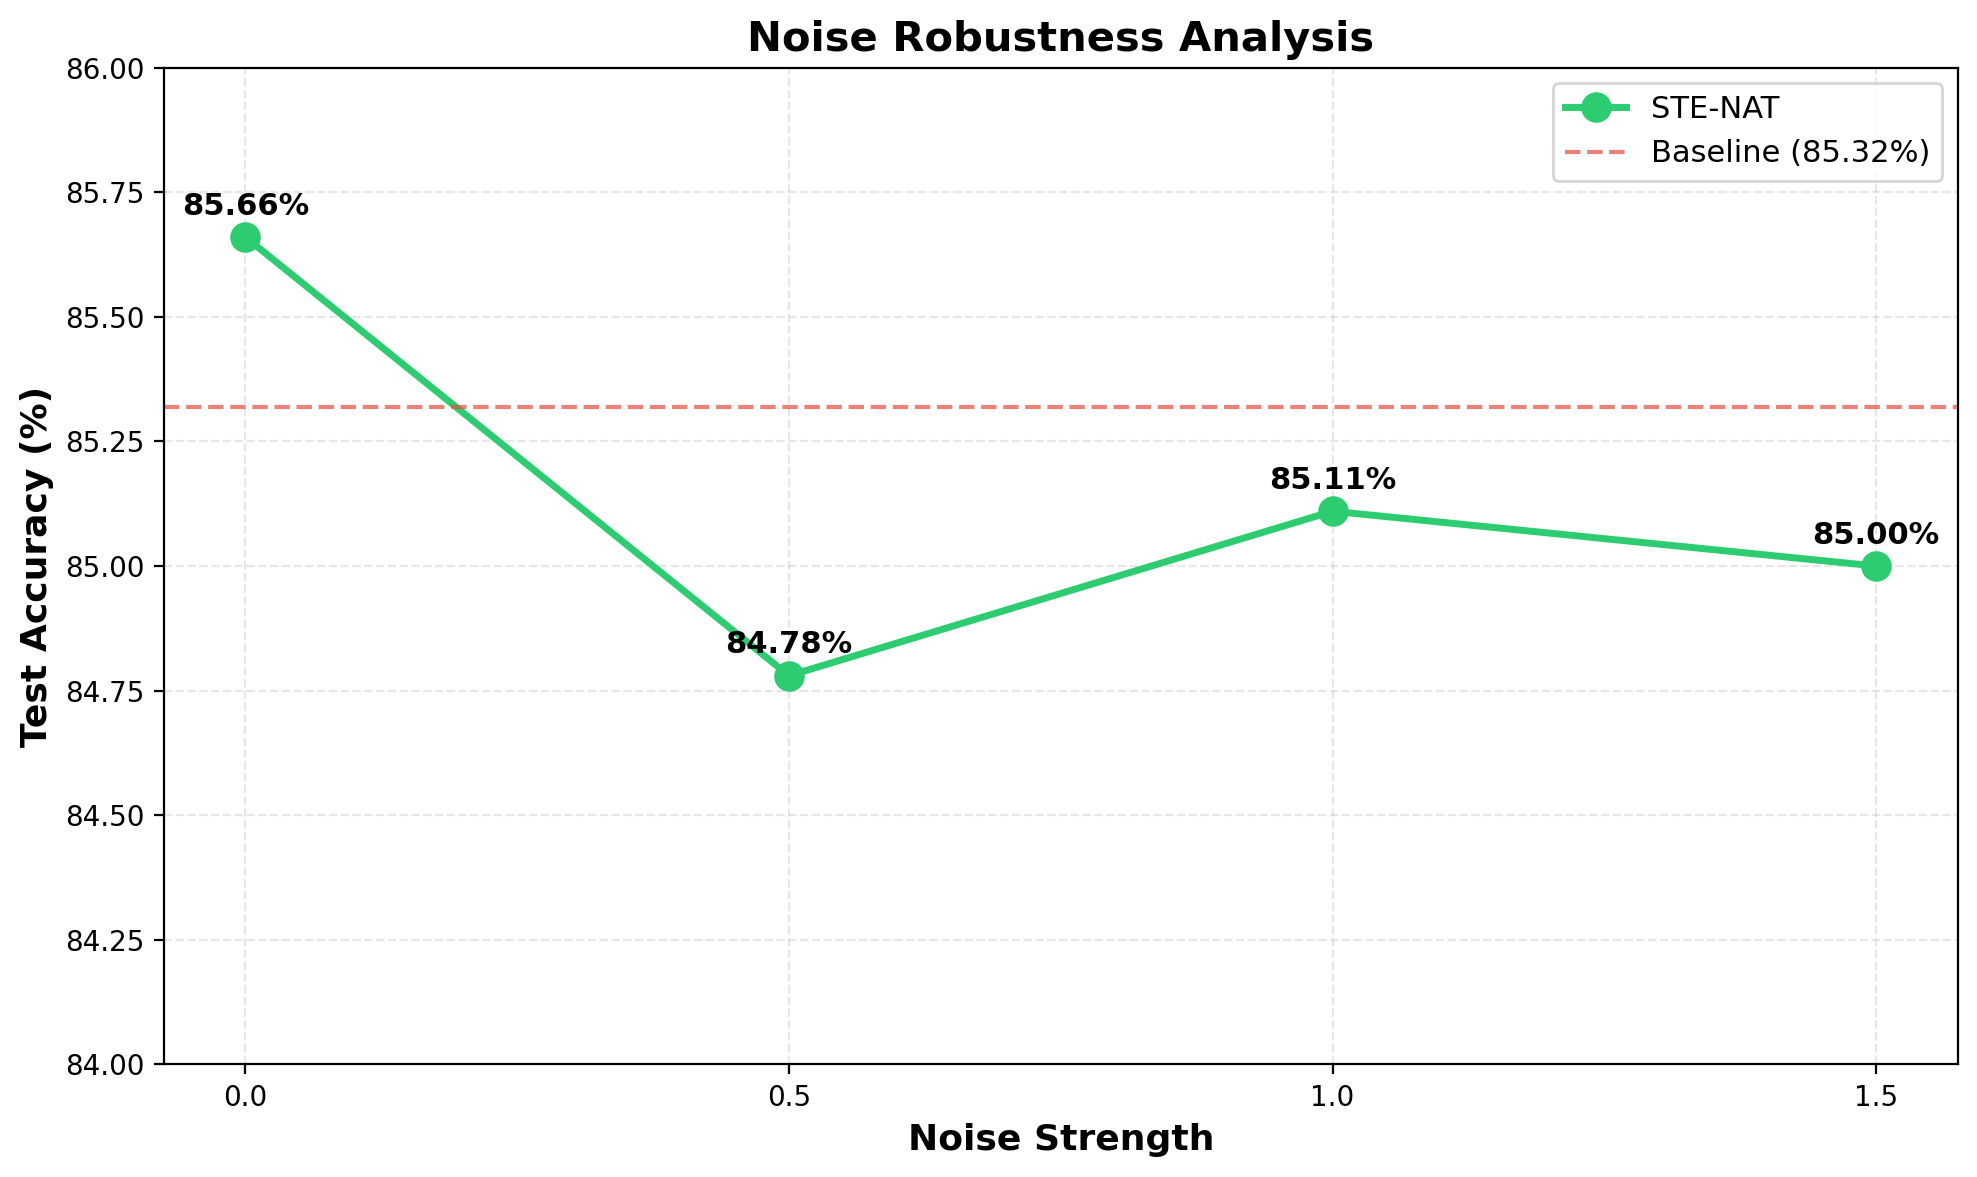
\includegraphics[width=0.85\textwidth,height=0.55\textheight]{../图表/图8_噪声鲁棒性.png}
\end{figure}
\end{frame}

% 第14页：消融实验
\begin{frame}{消融实验分析}
\begin{figure}
\centering
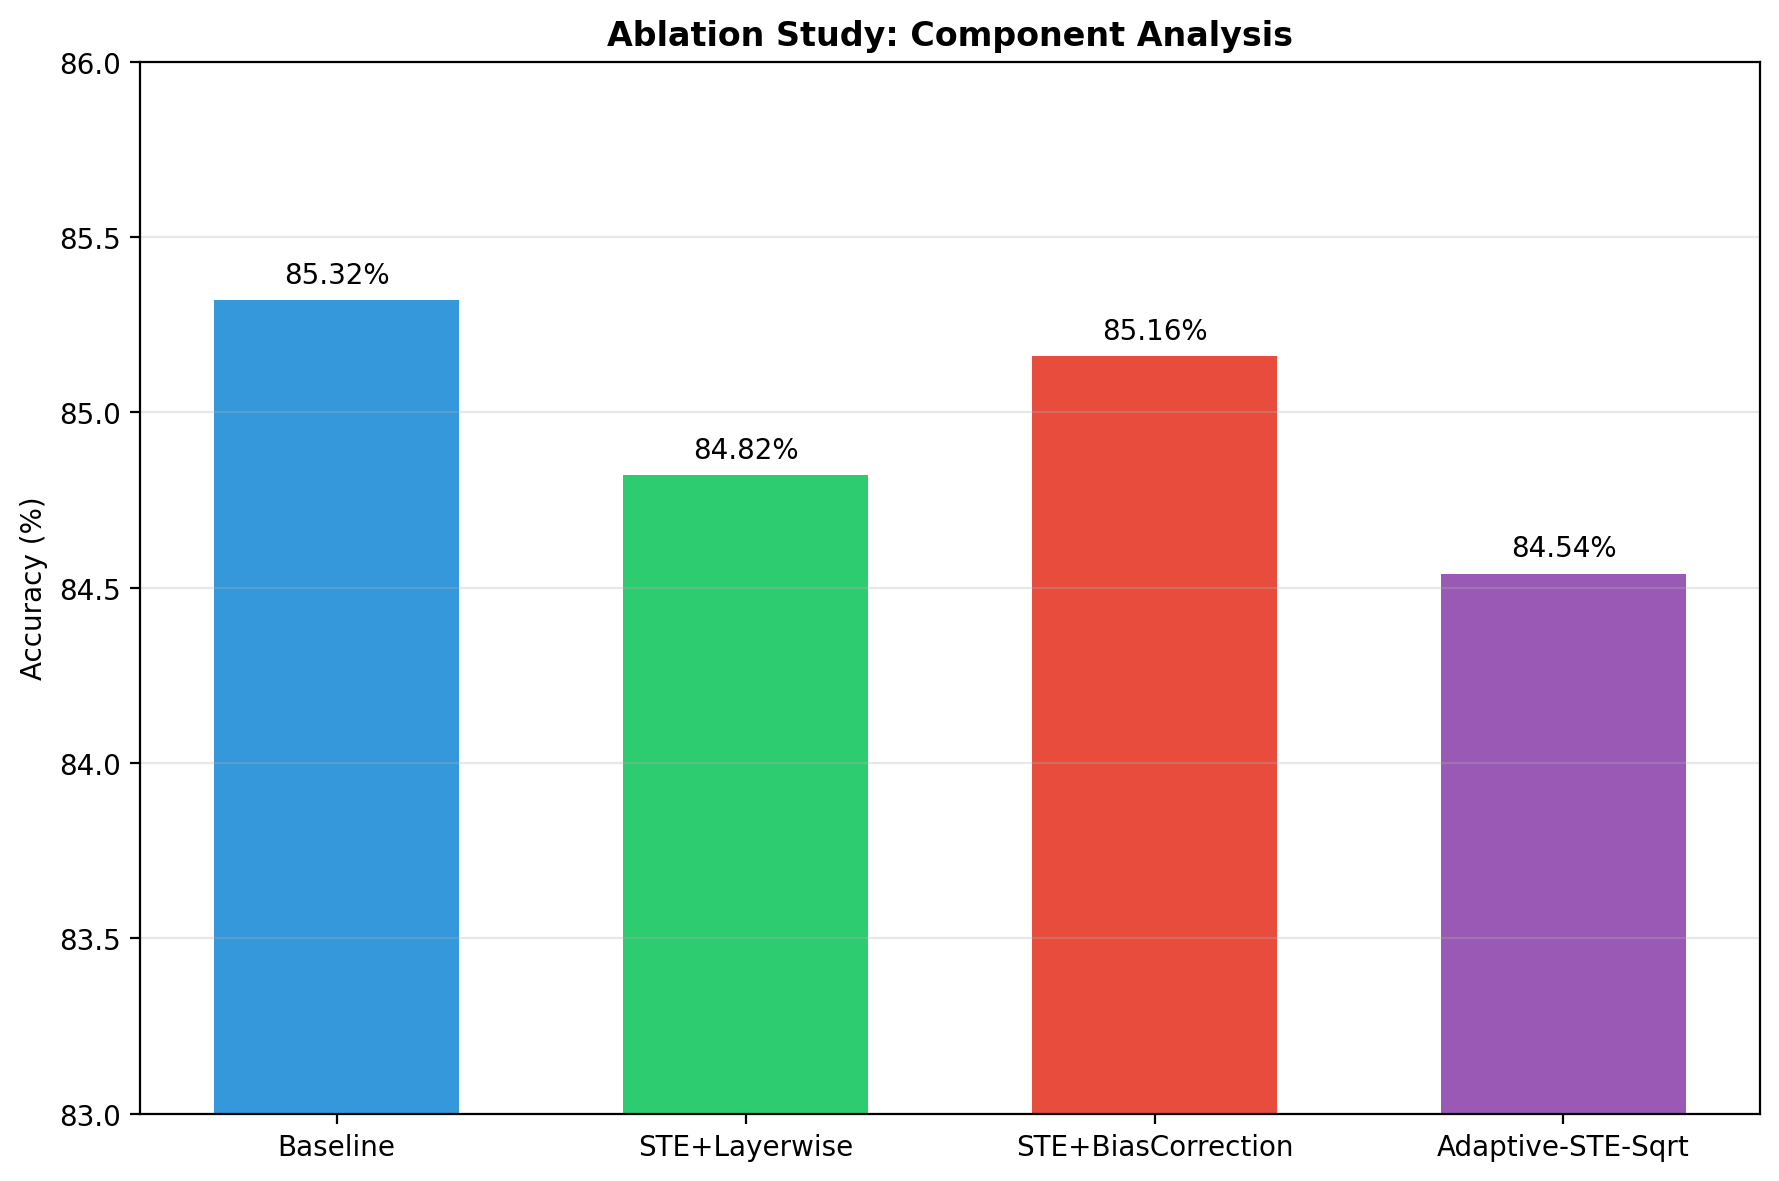
\includegraphics[width=0.85\textwidth,height=0.55\textheight]{../图表/图10_消融实验.png}
\end{figure}
\end{frame}

% 第15页：敏感性分析
\begin{frame}{敏感性分析}
\begin{figure}
\centering
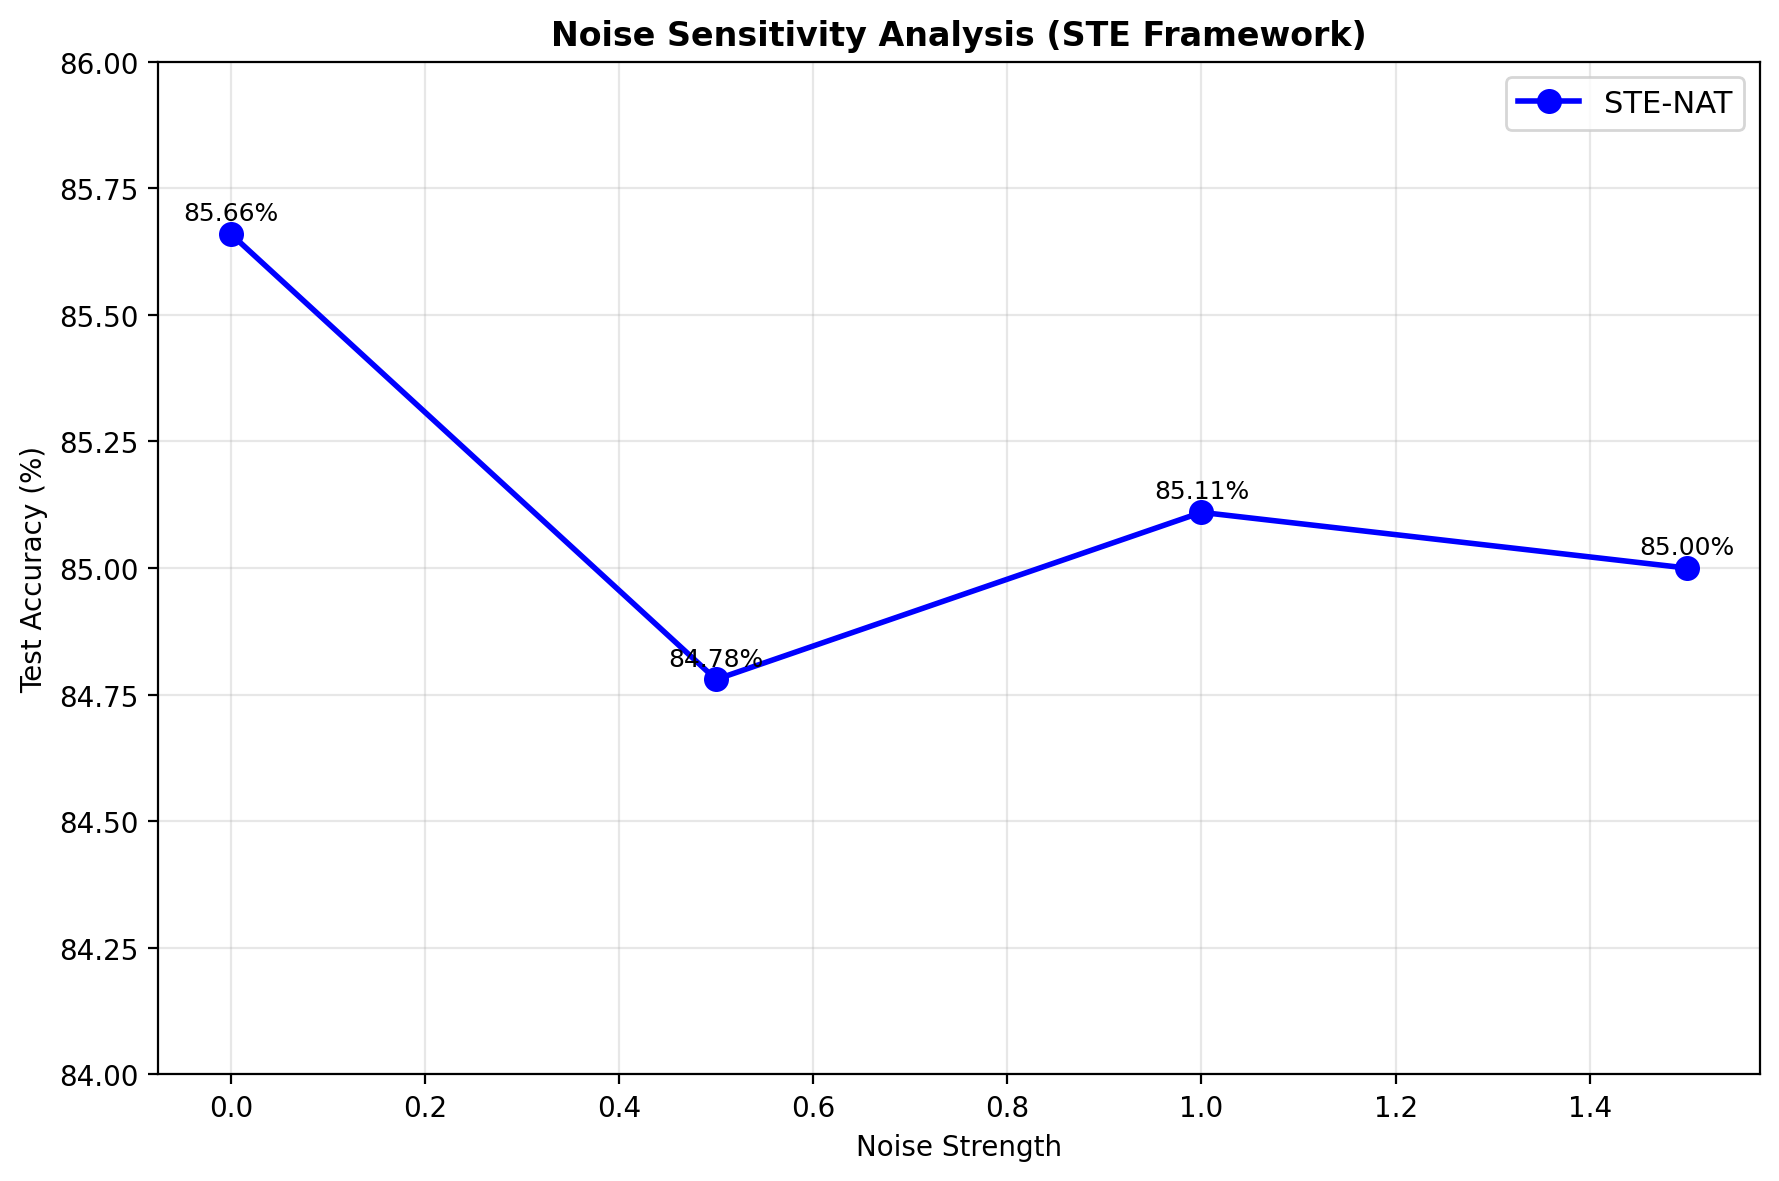
\includegraphics[width=0.85\textwidth,height=0.55\textheight]{../图表/图7_敏感性分析.png}
\end{figure}
\end{frame}

% 第16页：统计显著性
\begin{frame}{统计分析结果}
\begin{figure}
\centering
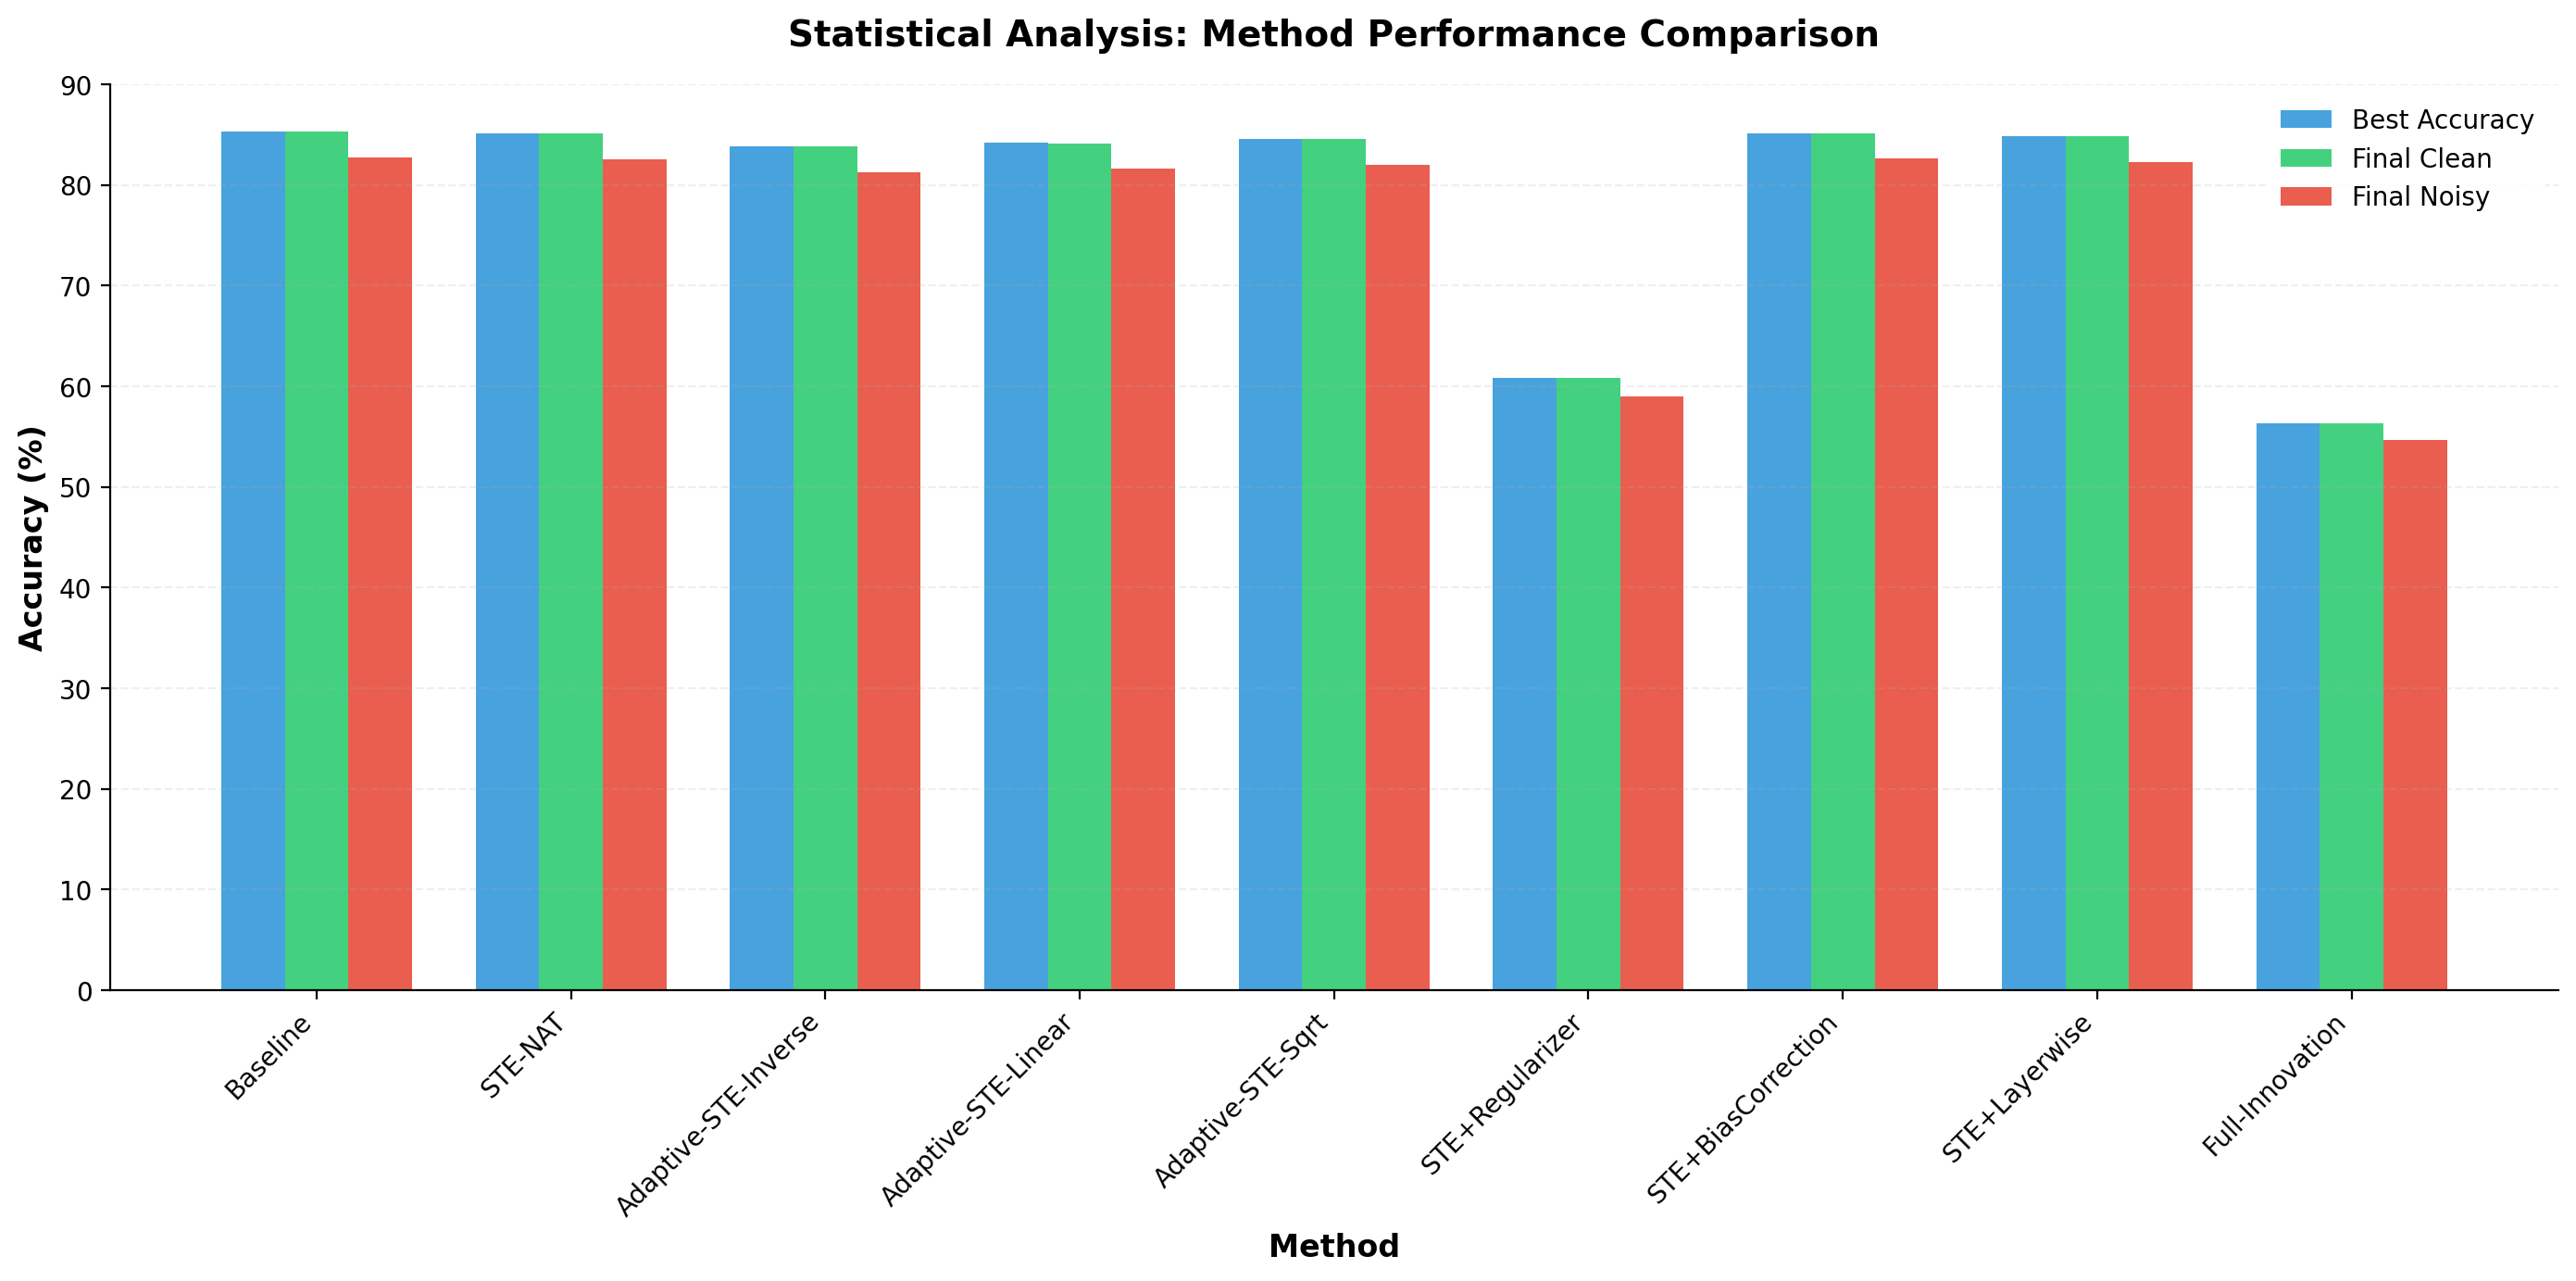
\includegraphics[width=0.85\textwidth,height=0.55\textheight]{../图表/图12_统计分析.png}
\end{figure}
\vfill
\tiny{t检验(p<0.05)和ANOVA验证方法间存在显著差异}
\end{frame}

% 第17页：创新点总结
\section{创新点总结}
\begin{frame}{主要创新点}
\begin{enumerate}
\item \textbf{自适应STE梯度估计}
\begin{itemize}
\item 根据实时噪声水平动态调整梯度缩放因子
\item 首次将自适应机制引入STE框架
\end{itemize}
\vfill
\item \textbf{Sqrt调度最优性证明}
\begin{itemize}
\item 从理论上证明Sqrt调度在MSE意义下的最优性
\item 实验验证其在各种噪声水平下的稳定性
\end{itemize}
\vfill
\item \textbf{EMA偏差校正机制}
\begin{itemize}
\item 使用指数移动平均估计真实梯度
\item 有效补偿梯度估计偏差
\end{itemize}
\vfill
\item \textbf{层次化噪声注入}
\begin{itemize}
\item 根据层深度自适应调整噪声强度
\item 提升整体网络的噪声鲁棒性
\end{itemize}
\end{enumerate}
\end{frame}

% 第18页：技术贡献
\begin{frame}{技术贡献}
\begin{block}{核心贡献}
\begin{itemize}
\item 提出完整的STE噪声感知训练框架
\item 验证自适应机制的有效性
\item 建立噪声-精度关系的理论分析框架
\item 为CIM芯片噪声鲁棒训练提供解决方案
\end{itemize}
\end{block}
\vfill
\begin{block}{应用价值}
可直接应用于实际CIM芯片的噪声感知训练，提升推理精度
\end{block}
\end{frame}

% 第19页：总结与展望
\section{总结与展望}
\begin{frame}{总结与未来工作}
\begin{columns}
\column{0.5\textwidth}
\begin{block}{工作总结}
\begin{itemize}
\item 成功实现基于STE的噪声感知训练框架
\item Adaptive-STE-Sqrt性能超越基准
\item 噪声鲁棒性显著提升
\end{itemize}
\end{block}
\column{0.5\textwidth}
\begin{block}{未来工作}
\begin{itemize}
\item 在更大数据集上验证（ImageNet）
\item 探索Tiki-Taka等先进模拟训练算法
\item 与真实CIM硬件协同设计
\end{itemize}
\end{block}
\end{columns}
\end{frame}

% 第20页：致谢
\begin{frame}{感谢聆听}
\vfill
\begin{center}
\Large\textbf{感谢评委老师的指导}
\end{center}
\vfill
\begin{center}
感谢主办方知存科技提供的平台
\end{center}
\vfill
\begin{center}
\Large{欢迎提问与交流}
\end{center}
\end{frame}

\end{document}
